\documentclass[11pt, a4paper]{report}
\usepackage[utf8]{inputenc}%codification of the document
\usepackage[french]{babel}
\usepackage{geometry}
\usepackage{times}
\usepackage{graphicx}
\usepackage{multicol}
\usepackage{float}
\usepackage{subcaption}
\usepackage{comment}
\usepackage{hyperref}
\usepackage{listings}
\usepackage{color}
\usepackage[dvipsnames]{xcolor}
\definecolor{EnoncerQuestions}{RGB}{10, 84, 68}
\definecolor{EnincerExercice}{RGB}{158, 19, 24}

\definecolor{lightgray}{rgb}{.98,.98,.98}
\definecolor{darkgray}{rgb}{.4,.4,.4}
\definecolor{blue}{rgb}{0.5, 0.2, 0.82}
\definecolor{purple}{rgb}{0.7, 0, 0.6}

\lstdefinelanguage{C}{
	keywords={typeof, new, true, false, catch, function, return, null, catch, switch, var, if, in, while, do, else, case, break},
	keywordstyle=\color{blue}\bfseries,
	ndkeywords={class, export, boolean, throw, implements, import, this},
	ndkeywordstyle=\color{darkgray}\bfseries,
	identifierstyle=\color{black},
	sensitive=false,
	comment=[l]{//},
	morecomment=[s]{/*}{*/},
	commentstyle=\color{blue}\ttfamily,
	stringstyle=\color{purple}\ttfamily,
	morestring=[b]',
	morestring=[b]"
}

\lstset{
	language=C,
	backgroundcolor=\color{lightgray},
	extendedchars=true,
	basicstyle=\footnotesize\ttfamily,
	showstringspaces=false,
	showspaces=false,
	numbers=left,
	numberstyle=\footnotesize,
	numbersep=9pt,
	tabsize=2,
	breaklines=true,
	showtabs=false,
	captionpos=b
}
\author{Badmavasan KIROUCHENASSAMY \& Caroline SCHMID}
\date{}
\title{Projet tutoré de Structures de Données - Graphes et Combinatoires : Problème du flot maximum}
\begin{document}
	\pagenumbering{roman}
	\begin{titlepage}
		\begin{center}
			
			\vspace*{1cm}
			
			\begin{figure}[h]
				\centering
				
\includegraphics[width=0.4\textwidth]{images/LOGO_Polytech-lille.jpg}
				\hspace{2cm}
				
\includegraphics[width=0.4\textwidth]{images/logo_ulille_transparent.png}
			\end{figure}
			
			\vspace*{2cm}
			
			\rule{1\textwidth}{.8pt}
			
			\LARGE{\textsc{Projet Informatique \& Statistique\\-\\Anti-monopoly}}
			
			\vspace*{1cm}
			
			\LARGE{\textsc{Rapport Final}}
			\vspace*{1cm}
			
			\small{IS2A3 - Mercredi 23 juin 2021}
			
			\vspace*{0.5cm}
			\rule{1\textwidth}{.10pt}
		
			\vspace*{2.352cm}
			
			\large{\textit{Encadrants :} Santiago BRAGAGNOLO\\Pablo TESONE}
			
			\vspace*{0.1cm}	        
			
			\large{\textit{Auteurs :} {Caroline SCHMID\\Brinda TSOBGNI}}
			
		\end{center}
	
	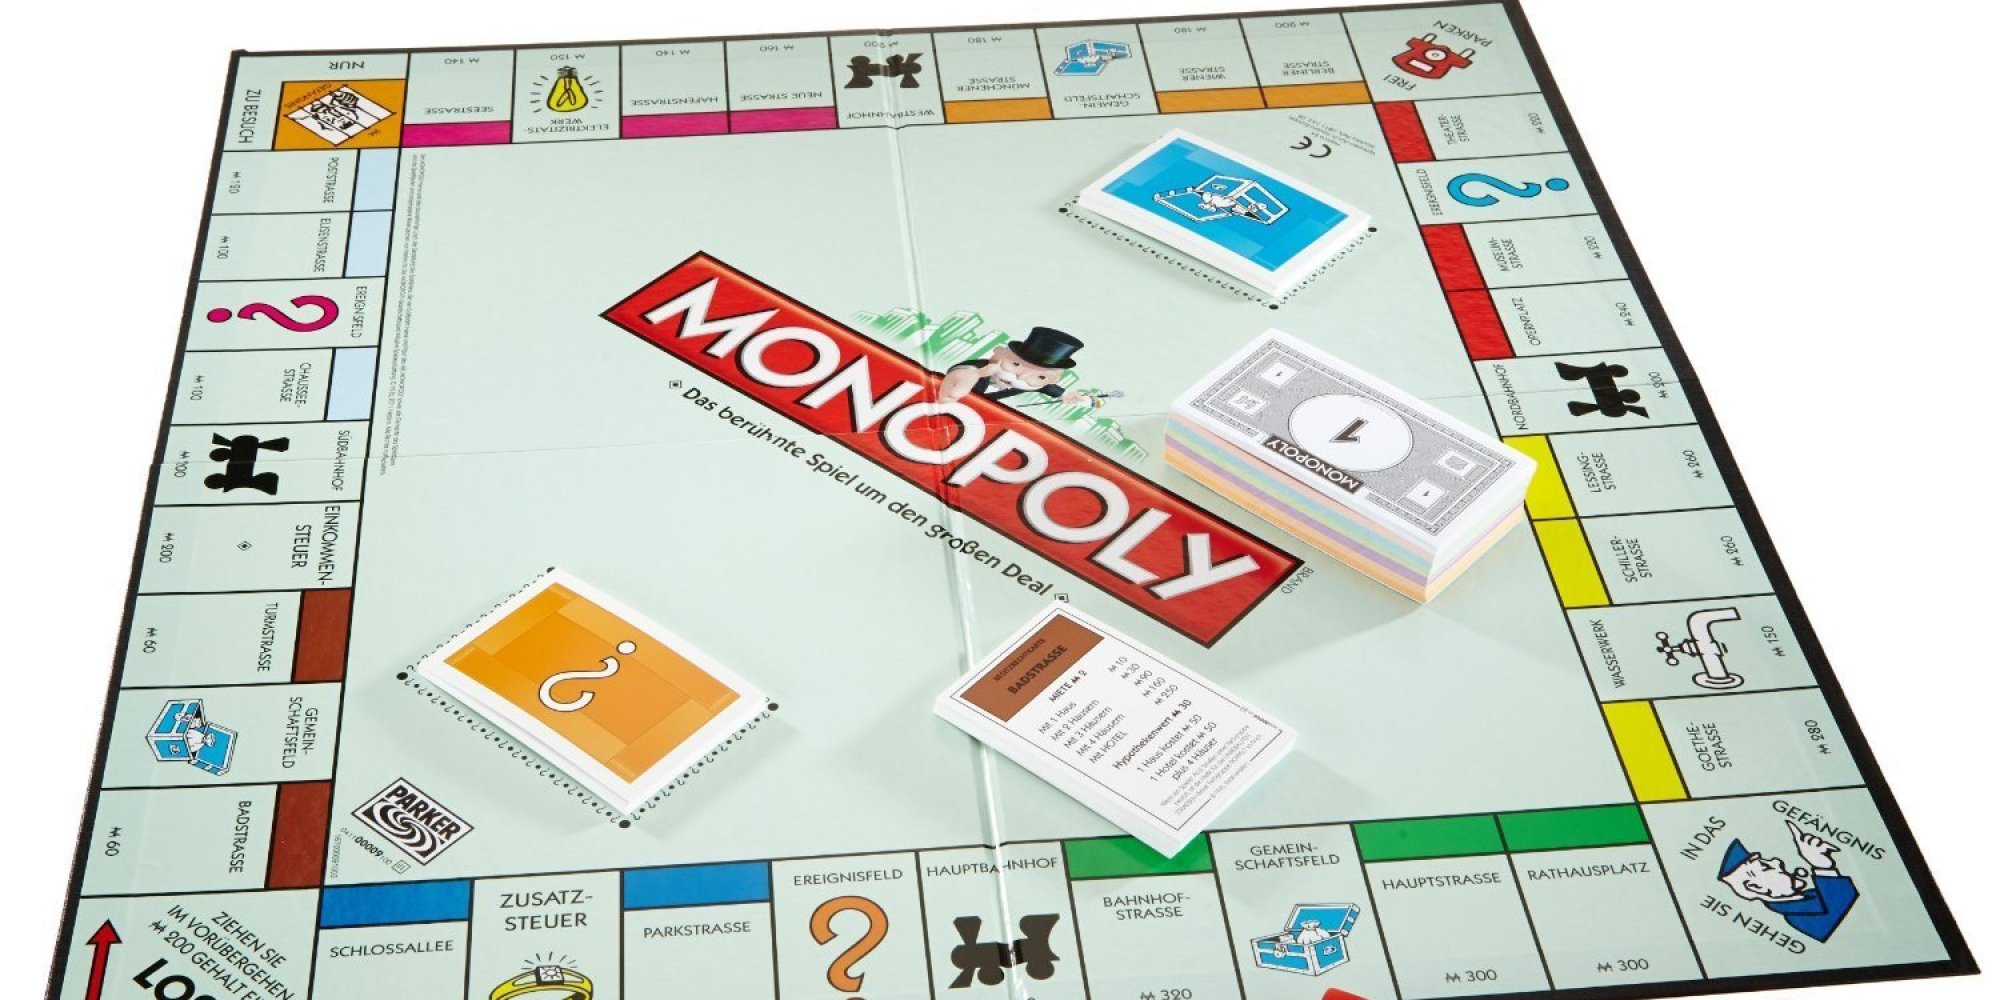
\includegraphics[width=0.2\textwidth]{images/MONOPOLY.jpg}
		
	\end{titlepage}
	
	
	%\setcounter{tocdepth}{2}
	\tableofcontents
	
	
	\chapter{Contexte du projet}
	\pagenumbering{arabic}
	
	Au cours de ce projet, on représente une partie de Monopoly dont la simulation est basée sur des joueurs pouvant être soit Prudents, soit Agressifs. L'un des joueur est l'État, il ne prend pas directement part au jeu mais en est un élément important.
	
	De plus, la construction du jeu dépend de la configuration que l'utilisateur choisit en lançant le programme. Ce choix détermine les valeurs des cases comme par exemple la valeur de la taxe à payer, mais également les moyens fournis aux différents joueurs en lançant le jeu, car dans certaines configurations les joueurs ne partent pas d'un même montant.
	
	Le plateau est constitué de cases de différents types, ces derniers déterminant les actions à réaliser en arrivant sur la case.
	
	Les joueurs sont caractérisés par leur style de jeu.
	
	La simulation crée les différentes entités nécessaires (un plateau, des joueurs, ...) et les fait jouer jusqu'à ce que soit l'État n'a plus de moyens, soit qu'il ne reste plus qu'un seul joueur sur le platau, voir aucun, ou encore que l'utilisateur décide de mettre fin à la partie.
	
	
	
	\chapter{Détail de la Simulation}
	
	La simulation peut être découpée en 3 étapes :
	
	\begin{enumerate}
		
		\item Initialisation du jeu
		
		\item Déroulement du jeu
		
		\item Résultats
	
	\end{enumerate}
	
	
	\section{Initialisation du jeu}
	
	On demande à l'utilisateur d'indiquer :
	
	\begin{enumerate}
		
		\item la configuration dans laquelle il veut lancer la simulation
		
		\item le nombre de joueurs pour chaque style de jeu
		
	\end{enumerate}
	
	Le plateau ainsi que la liste des joueurs sont créés en fonction des informations indiquées et de paramtres préenregistrés dépendant du mode de simulation choisi. L'État est également ajouté à la liste des joueurs mais est traîté de manière différente des autres joueurs.
	
	\section{Déroulement du jeu}

	Le jeu se déroule de la manière suivante : chaque joueur joue à tour de rôle jusqu'à ce que la fin de la partie soit déclarée. Pour chaque joueur, sauf l'État, le dé est lancé, donnant un résultat de 1 à 6. le joueur qui a la main avance d'autant de cases et réalise l'action indiquée dessus. Les actions peuvent être les suivantes :

	\begin{itemize}
		
		\item Si la case est un investissement et si l'investissement n'est pas encore la propriété d'un joueur, s'il appartient à l'État, le joueur peut décider de l'acheter ou pas, dépendant de son style de jeu et de ses moyens. Si l'investissement appartient déjà à un autre joueur, celui qui joue son tour doit payer au propriétaire un pourcentage de la valeur de l'investissement.
		
		\item Si la case est une loi antitrust et si les propriétés du joueur dépassent un seuil fixé par l'État, il doit revendre certaines de ses possessions à moitié prix à l'État pour se trouver en dessous de ce seuil. Le joueur, dépendant de son mode de jeu choisira les propriétés dont il veut se séparer.
		
		\item Si la case est un bureau des finances publiques, le joueur doit payer une taxe sur la somme d'argent qu'il a. La taxe est d'un certain pourcentage indiqué dans la case et est à payer à l'État.
		
		\item Si la case est une subvention, le joueur reçoit de l'État le montant indiqué dans la case.
		
		\item Si la case est une case de repos, le joueur ne fait rien.
		
	\end{itemize}
	Un joueur sort du jeu s'il n'a plus de moyen financier. Ça se matérialise par un entier passant de $0$ (le joueur est encore dans le jeur) à un entier suppérieur, permettant de retrouver l'ordre dans lequel les joueurs sont sortis.\\
	Le jeu prend fin si l'une des conditions suivantes est remplie :
	
	\begin{enumerate}
		
		\item Il ne reste plus qu'un seul ou aucun joueur sur le plateau.
		
		\item L'État n'a plus de moyen financier, il a échoué.
		
		\item L'utilisateur décide d'interrompre la partie.
		
	\end{enumerate}
	
	
	\section{Résultats}
	
	En premier est affiché la raison pour laquelle le jeu a été interrompu.
	
	Les résultats sont affichés par ordre : sont indiqués, le vainqueur, le montant de ses investissements, ses moyens financiers et son patrimoine ; puis vient le tour du second avec les mêmes informations et ainsi de suite.
	
	
	
	\chapter{Schéma UML des classes}
	
	\begin{figure}[h]
		\centering
		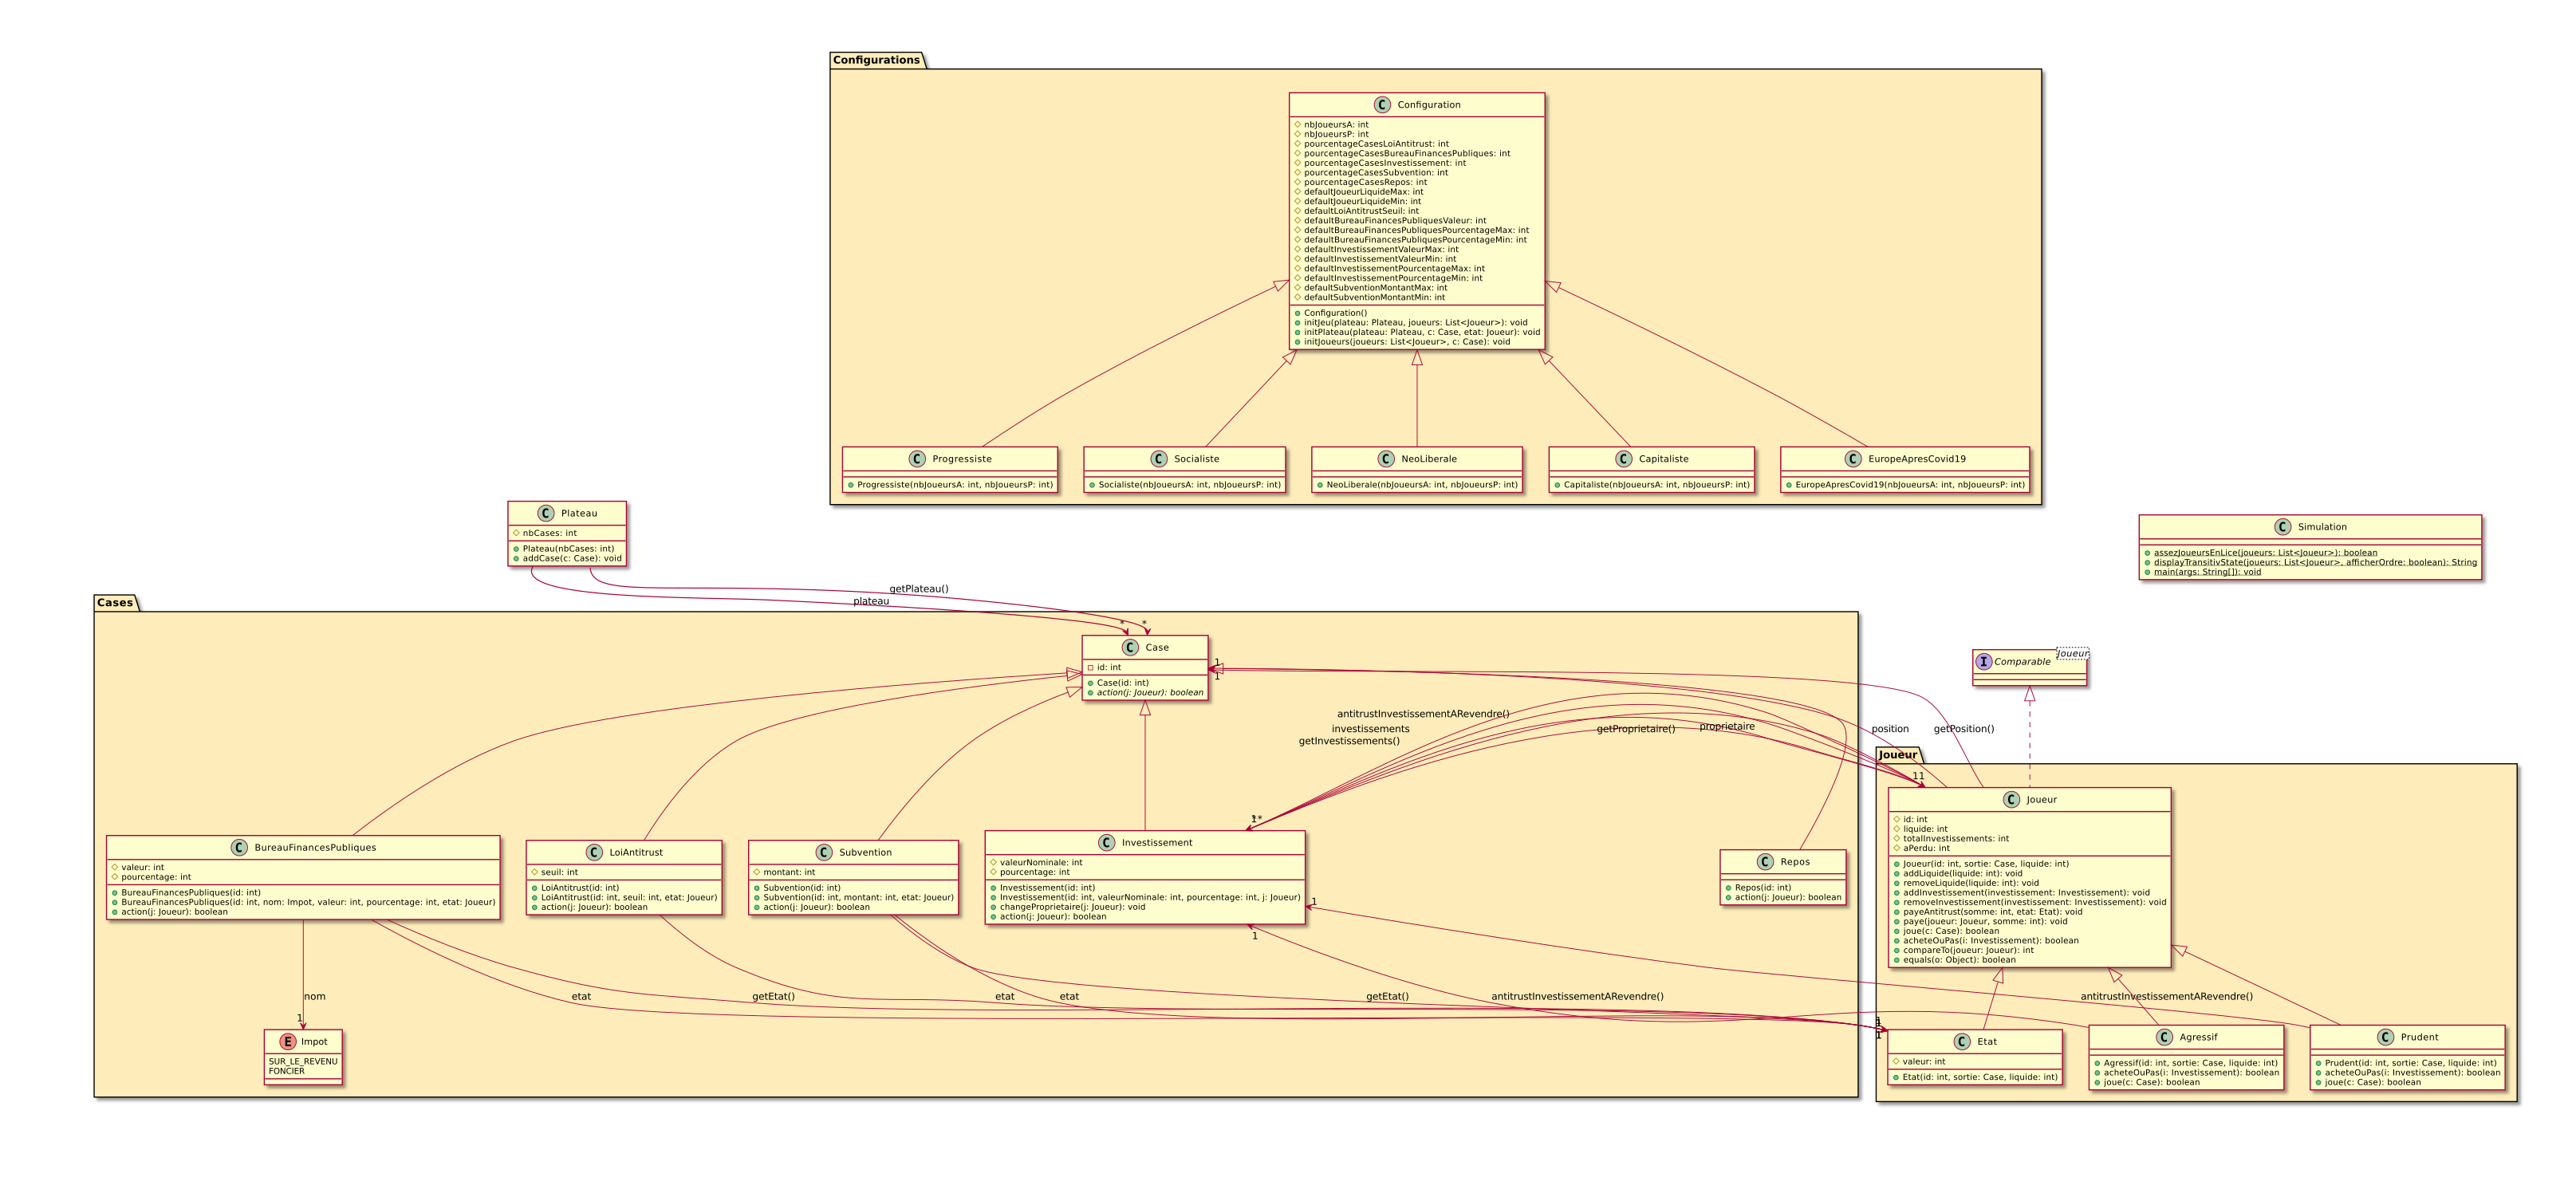
\includegraphics[width=1.1\textwidth]{images/umlFin.png}
	\end{figure}

	\pagebreak
	
	Toute les classes sont regroupées dans un package \verb|Monopoly|.
	
	Le projet est découpé en 5 sous-structures :
	
	\begin{itemize}
		\item Le package \verb|Cases| contenant les différents types de cases, chacun représenté par une classe, toutes héritant de la classe \verb|Case|, classe abstraite permettant d'indiquer que tous ces types sont des cases.\\
		\begin{center}
			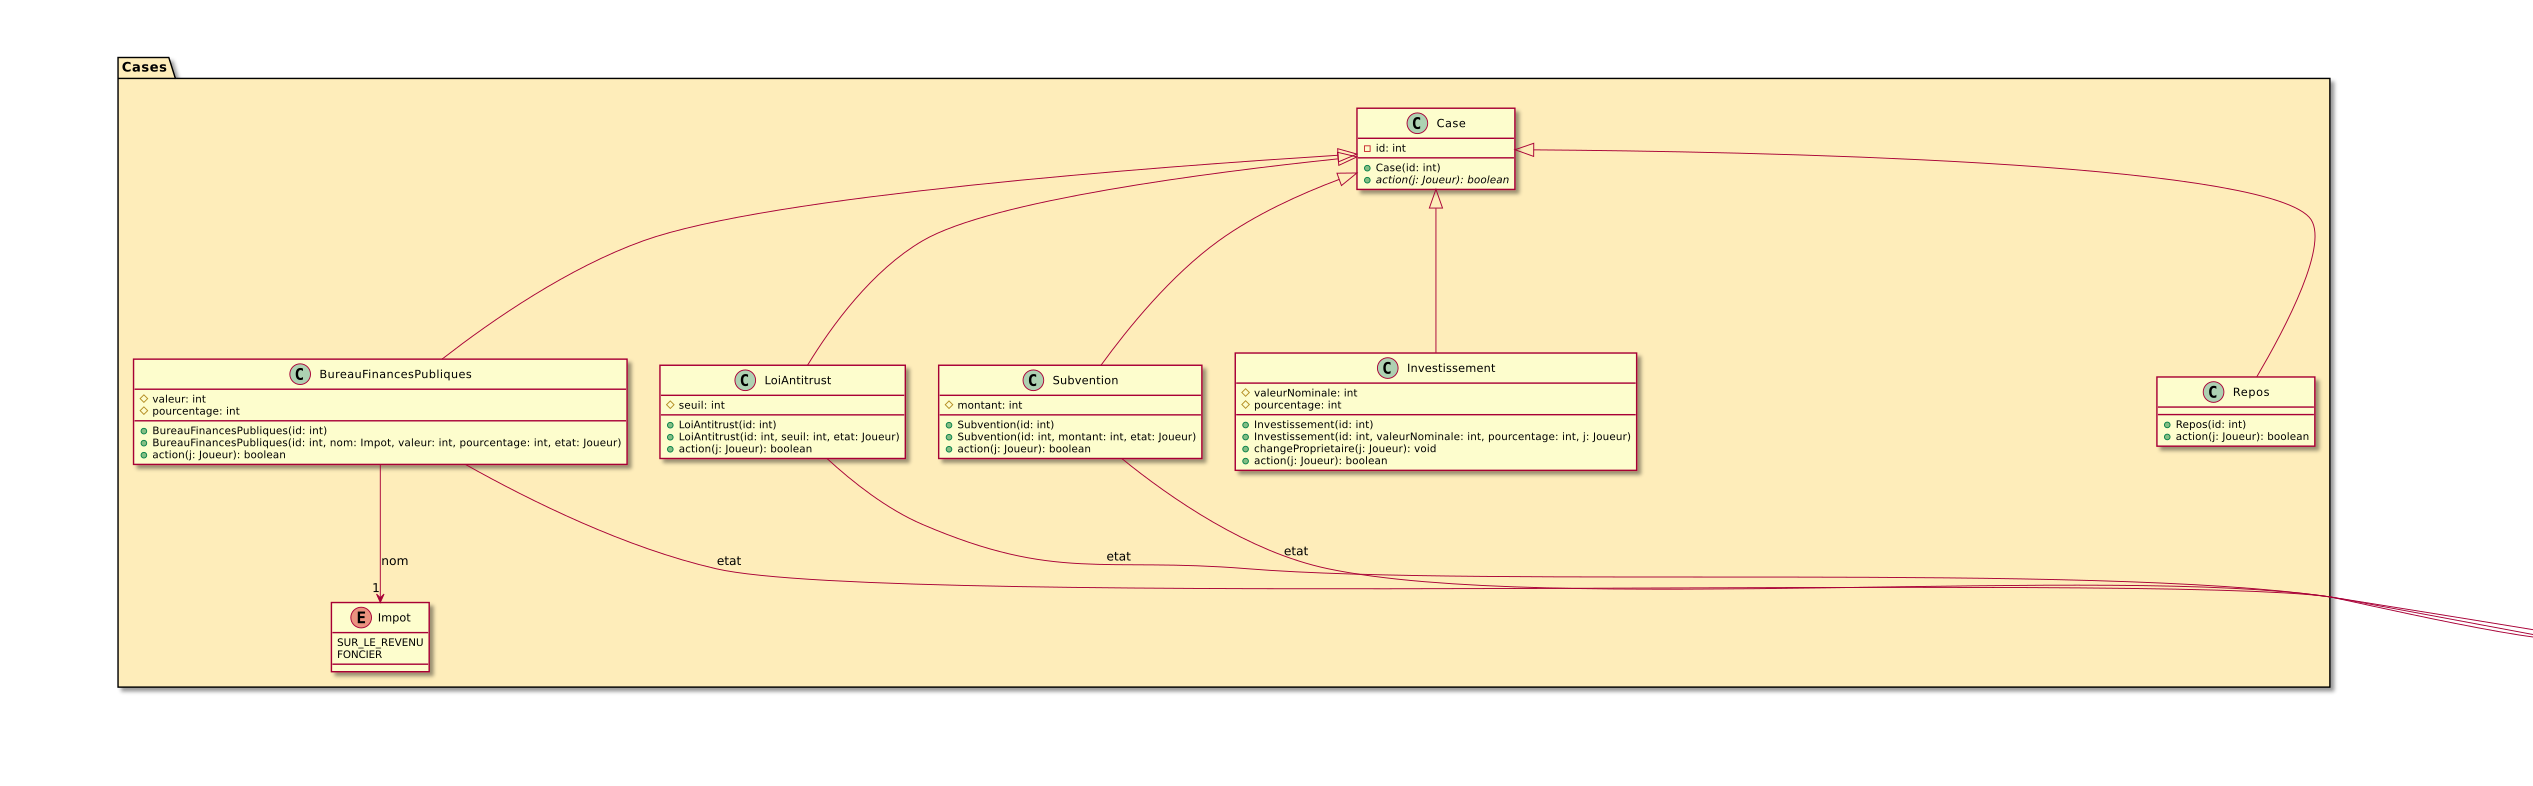
\includegraphics[width=1\textwidth]{images/UMLCases.png}\\
		\end{center}
		
		\item Le package \verb|Joueurs| contenant les différents styles de jeu, chacun représenté par une classe dont la classe \verb|Etat|, toutes héritant de la classe \verb|Joueur|, classe abstraite permettant d'indiquer que tous ces styles sont des joueurs.\\
		\begin{center}
			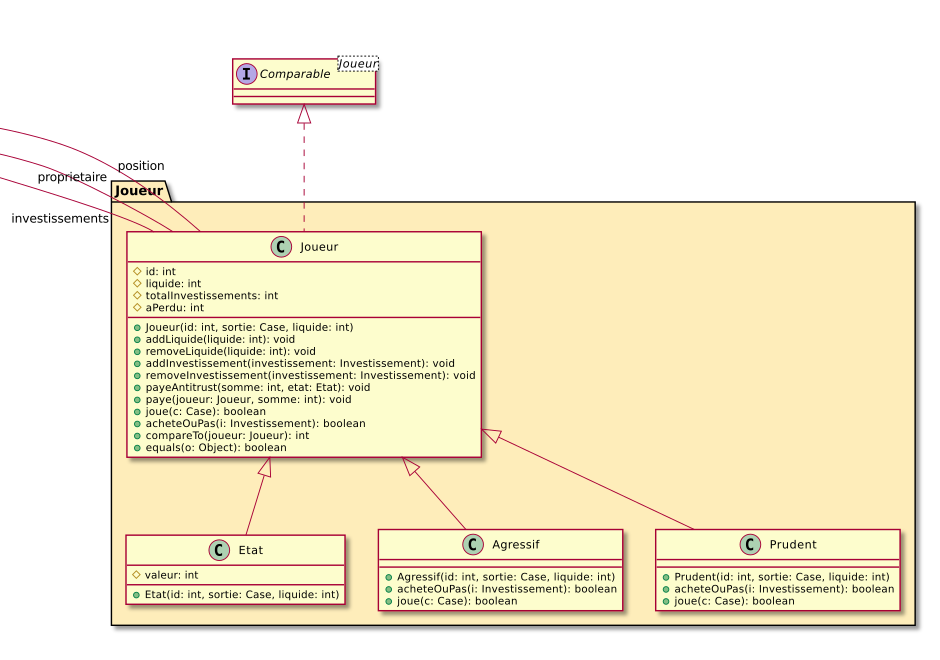
\includegraphics[width=1\textwidth]{images/UMLJoueurs.png}\\
		\end{center}
		
		\pagebreak
		
		\item Le package \verb|Plateaux| contient pour le moment qu'une classe \verb|Plateau| permettant de construire le plateau et d'accéder à ses attributs. Une extension serait possible en ajoutant d'autres plateaux.\\
		\begin{center}
			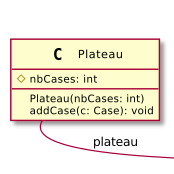
\includegraphics[width=0.15\textwidth]{images/UMLPlateaux.png}\\
		\end{center}
		
		\item Le package \verb|Configurations| contenant les différents environnements dans lequels le jeu peut se dérouler, chacun représenté par une classe, toutes héritant de la classe \verb|Configuration|, classe abstraite permettant d'indiquer que tous ces types sont des configurations.\\
		\begin{center}
			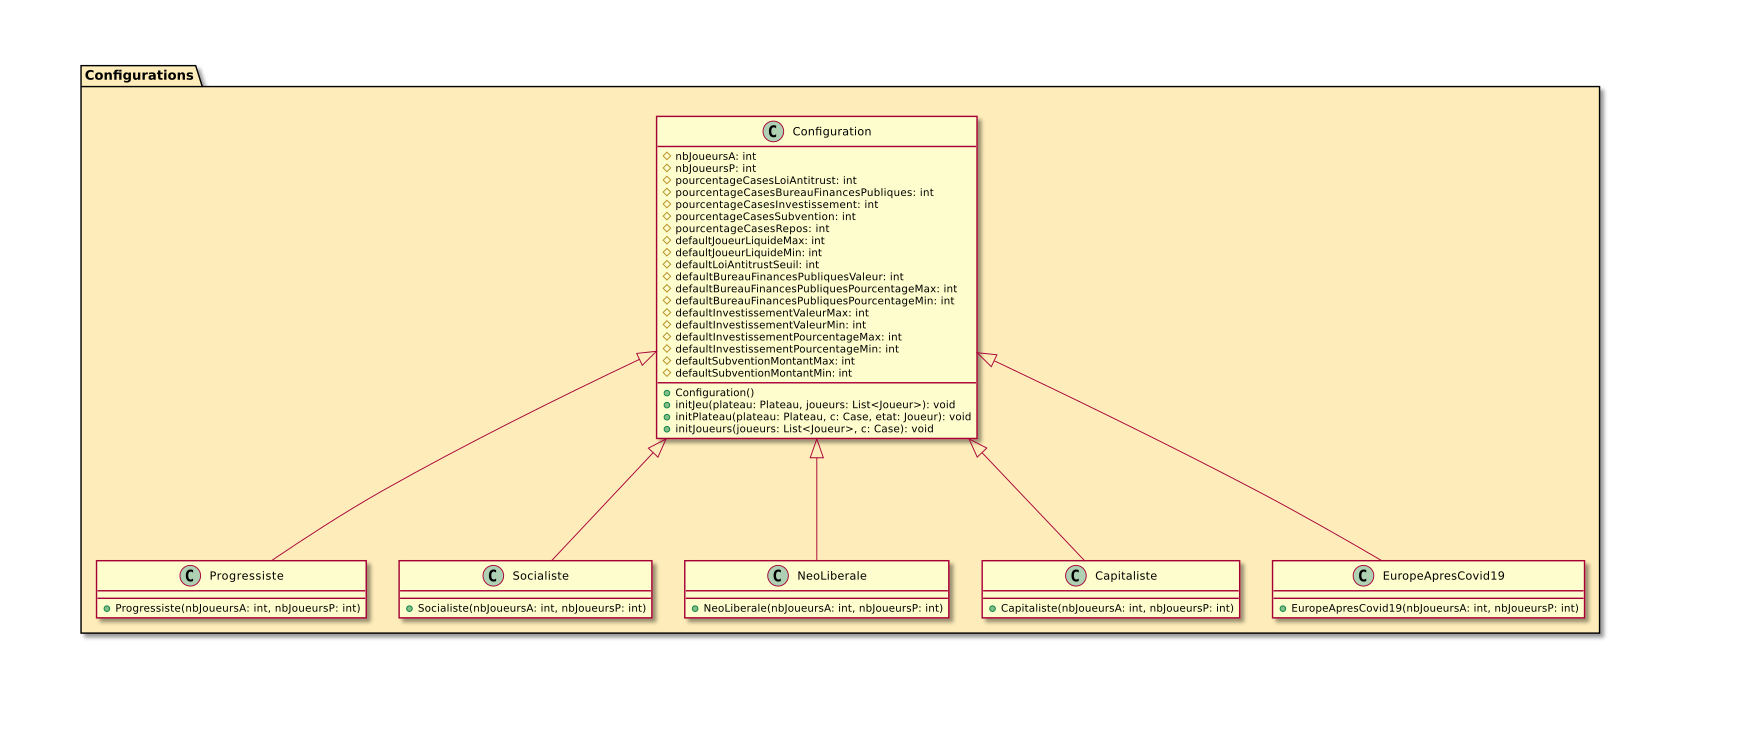
\includegraphics[width=1\textwidth]{images/UMLConfigurations.png}\\
		\end{center}
		
		\item La classe \verb|Simulation|, le main. Contient la création, le déroulement et la fin du jeu.\\
		\begin{center}
			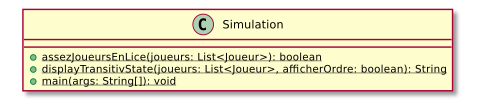
\includegraphics[width=0.5\textwidth]{images/UMLSimulation.png}\\
		\end{center}
		
	\end{itemize}
	
	
	\chapter{Choix des structures de données non-primitives}
	
	La structure non-primitives de la librairie $java.util$ mise en œuvre est la '$LinkedList$'. Elle sert à contenir le plateau, les joueurs ainis que les investissements de chaque joueur.
	
	Le choix de la $LinkedList$ a été fait car les $tableaux$ et $ArrayList$ sont moins efficaces du point de vue de l'ajout et suppression d'éléments.
	
	
	\chapter{Tests Unitaires}
	
	Un test unitaire peut être réalisé par nombre de méthodes dans la classe, autres que constructeur, getteurs, setteurs, égalités, comparaisons, affichage.
	
	Les tests unitaires peuvent être réalisés par package.
	
	La classe Simulation contient une méthode de vérification de la constitution de la liste des joueurs, on peut vérifier que celle-ci renvoit la bonne conclusion.
	
	\section{Cases}
	
	Le package \verb|Cases| : la méthode $action$ peut être testée pour vérifier que l'action liée à la case est effectuée correctement.
	
	\section{Joueurs}
	
	Le package \verb|Joueurs| : les méthode d'achat, $joue$ et $acheteOuPas$ peuvent être testées. Certaines, comme $joue$ nécessiteront plusieurs tests pour s'assurer que l'action a été réalisée correctement.
	
	\section{Plateaux}
	
	Le package \verb|Plateaux| : le plateau ne présente aucune méthode intéressante à tester étant donné qu'il sera construit dans une classe de configuration.
	
	\section{Configurations}
	
	Le package \verb|Configurations| : chaque classe de ce package ne contient aucune méthode sauf la classe \verb|Configuration| construisant aussi bien la liste des joueurs et le plateau, en fonction des demandes de l'utilisateur et des valeurs contenues dans cette classe et celle e la configuration demandée par le joueur. ces méthodes peuvent difficilement être testées étant donnée qu'elles dépendent fortement de l'aléatoire pour que chaque jeu soit différent.
	
	
	\chapter{Changements réalisés}
	
	Les changements opérés entre le premier rapport et l'implémentation sont les suivants :
	
	\begin{itemize}
		\item Simulation : la simulation n'est plus uniquement constituée du main, mais également d'une méthode d'affichage de l'état de la liste des joueurs et une méthode vérifiant s'il y a encore plus d'un joueur apte à jouer dans la liste des joueurs initiaux (hors État).
		 
		\item Cases : ajout de la méthode $action$ réalisant l'action du joueur dépendant de son caractère et de la case sur laquelle il est tombé. Ce changement permet de déléguer à chaque case l'action et alléger la fonction joue. Ça permet d'éviter les $instanceof$.
		
		\item Joueurs : pour qu'un joueur paye un montant à un autre joueur et éviter de changer les attributs à partir d'une classe extérieur, cette méthode mise en place.
		Les classes \verb*|Agressif| et \verb*|Prudent| implémentent également une méthode $acheteOuPas$ pour indiquer si, selon leur caractère, ils achètent l'investissement en paramètre ou pas.
		
		\item Plateaux : le plateau n'a pas subi de modifications majeurs à mentionner.
		
		\item Configurations : $initPlateau$ et $initJoueurs$ permettent d'alléger la méthode $initJeu$. Ces deux méthodes sont respectivement grandes donc mettre leur code dans une seule méthode la rendrait vraiment très grande, donc difficilement testable, ce qui entraine d'autant plus d'erreurs.
		Des attributs ont également étés ajoutés, correspondant aux valeurs possibles pour les différentes cases et les montants attribués aux joueurs en lancement de jeu. Les valeurs pouvant varier d'une case à l'autre sont représentées par deux attributs constituant un interval dans lequel les valeurs attribuées aux cases vont se trouver, choisies par de l'aléatoir.
		
	\end{itemize}


	\chapter{Améliorations pouvant être apportées}
	
	$initPlateau$ et $initJoueurs$ pourraient être séparés en plusieurs plus petites méthodes pour pouvoir les tester plus aisément.
	
	De plus, il serait intéressant de dispercer ces morceaux dans les classes appropriées : la construction des cases de subvention dans la calsse \verb*|Subvention|, les joueurs Prudents dans la classe \verb*|Prudent| et ainsi de suite. La méthode $initJeu$ peut rester dans la classe \verb*|Configuration| mais déplacer la méthode $initJoueurs$ appelant les nouvelles méthodes de constructions des différents Joueurs dans la classe \verb*|Joueur| et chaque méthode de construction de joueur dans sa classe respective. De même, déplacer la méthode $initPlateau$ dans la classe \verb*|Plateau| et les méthodes de construction de chaque case dans leurs classes respectives. Cette dernière méthode peut peut-être être une méthode de la super-classe \verb*|Case| réalisant la boucle et permettant un $@Override$ dans les classes de chaque case. Ce sera une méthode $abstract$ sinon.
	
	
	\chapter*{Conclusion}
	\pagenumbering{Alph}
	
	Ce projet nous a permis de mettre en application les notions de Programmation Orientée Objet qui nous ont été enseignées en cours et mettre à l'épreuve nos connaissances fraichement acquises ainsi que la réalisation d'un projet.
	
	Le niveau était très haut et les niveaux le connaissances très différents mais en apportant chacune ses connaissances et son avis, nous sommes arrivées au terme de ce projet avec un programme qui tourne et répond aux attentes.
	
	Nous avons essayé de prendre en compte des contraintes de programmation comme l'espace mémoire et le temps d'exécution pour optimiser notre programme et le rendre le plus efficace et lisible possible et adhérant au mieux au paradigme Orienté Objet.
	
	
\end{document}
